\section{Background}
    Assessing community resilience involves a multifaceted process, considering numerous interrelated factors, including infrastructure, social dynamics, environmental conditions, and economic stability \cite{community_resilience_group_community_2015,community_resilience_group_community_2015-1}. This assessment process is inherently fraught with uncertainties stemming from the complex interplay of numerous factors. Among these uncertainties, one pivotal source is the nature of the hazard itself. Hazards come in various forms and intensities, and their occurrence is governed by probabilistic processes that introduce inherent uncertainty. In the context of flood hazards, the traditional deterministic approach, such as using a 100-year flood scenario for design, has been replaced by a probabilistic approach that acknowledges the inherent uncertainty in flood hazards \cite{quagliolo_experimental_2021,bulti_community_2019,eslamian_flood_2023,winter_event_2020}. Similarly, seismic hazard assessment has moved away from relying on a single deterministic scenario \cite{tantala_earthquake_2008,cardona_seismic_1997,faccioli_study_1999} toward probabilistic seismic hazard analysis \cite{gerstenberger_probabilistic_2020,campbell_seismic_2002}. 
    
    Sometimes, the worst-case scenario is considered the representative hazard scenario. However, opting to design exclusively for worst-case scenarios is not always the most effective strategy. It can lead to excessive costs and overly conservative measures unless dealing with critical structures like levees or dams, where potential damage could incur significant expenses. Moreover, determining the true worst-case scenario is often a complex endeavor, especially when dealing with multifaceted hazards. For instance, in seismic hazard analysis, the largest magnitude earthquake does not necessarily equate to the most destructive event. This concept can be illustrated through a hypothetical scenario involving a site with two linear sources, as depicted in Figure~\ref{fig:DSHA}. In this figure, it is evident that an earthquake source with a lower magnitude and situated closer to the site produces a more intense measurement over a shorter duration compared to an earthquake source with a higher magnitude located farther away from the site.

         \begin{figure}[H]
        \centering
        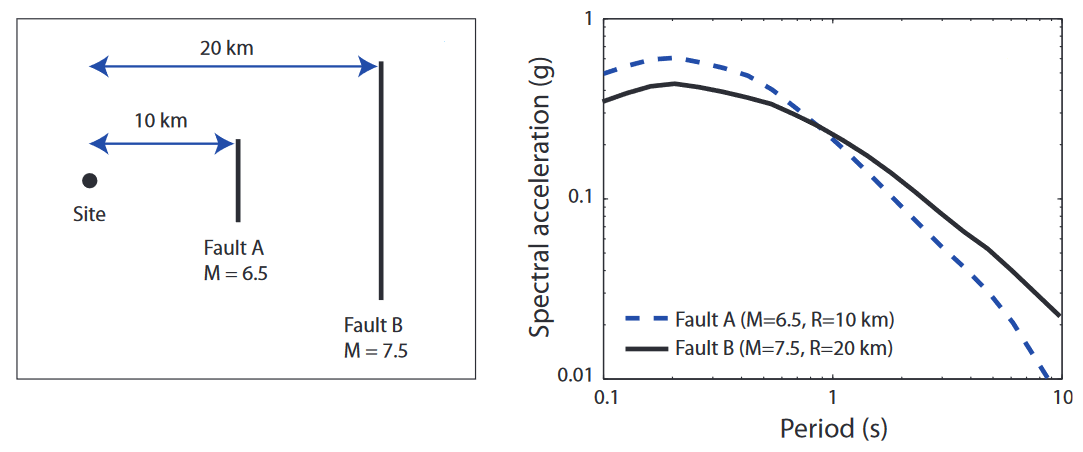
\includegraphics[scale=0.5]{Figures/Images/Background/DSHA.png}
        \caption{Predicted median response spectra from the two earthquake events (prediction obtained from the model of \cite{campbell_nga_2008})}
        \label{fig:DSHA}
    \end{figure}
 
    Various techniques have been used in the literature to address uncertainty in hazard assessment and generally in resilience planning. A comprehensive review of these techniques is provided in \cite{sun_resilience_2020}. Among these techniques, simulation is the most commonly used method \cite{sun_resilience_2020} and in particular, MC simulation has gained widespread recognition to address uncertainty \cite{zheng_bayesian-based_2022, cicilio_electrical_2020, tabandeh_uncertainty_2022, younesi_assessing_2020}. MC simulation involves the generation of numerous random samples or scenarios to estimate complex phenomena. Due to its flexibility and versatility, MC simulation is widely applied in community resilience assessment.

    However, MC simulation encounters a significant challenge when dealing with low-probability, high-consequence events. These rare but impactful occurrences, such as extreme earthquakes or severe pandemics, can considerably increase the variance of MC estimations. Consequently, this presents a challenge in obtaining reliable estimates for the likelihood and impact of such events.
    
    To mitigate this challenge, the concept of importance sampling emerges as a valuable tool. Importance sampling is a variance reduction technique that seeks to focus computational effort on the regions of interest within the probability distribution. By systematically biasing the random sampling towards events of greater significance, importance sampling enhances the accuracy and efficiency of MC simulations \cite{melchers_importance_1989, heinkenschloss_conditional-value-at-risk_2018}.
    
    The importance density function, a crucial element of importance sampling, plays a pivotal role in guiding the sampling process. It defines the probability distribution from which samples are drawn, emphasizing events that have greater relevance in the analysis. This ensures that computational effort is concentrated where it matters most.

    The effectiveness of IS-based approaches relies heavily on constructing the importance density function properly; otherwise, a significant number of samples may still be required. The importance density function can be manually defined, termed manual-IS in this paper. However, it's not always clear how to define a proper importance density function, particularly in high-dimensional problems where reducing the variance of estimation is crucial. To address this challenge, various adaptive IS techniques have been developed to iteratively approach the optimal importance density function \cite{tomasson_improved_2017, depina_coupling_2017, ching_efficient_2009, chaudhuri_information_2020, aslam_ansari_data-driven_2020}. Among these techniques, MCMC-IS is a notable implementation. In this paper, we visually compare the performance of MC simulation, manual-IS, and MCMC-IS techniques through a numerical example, particularly when dealing with rare and high-consequence events. This comparison aims to provide insights into their relative effectiveness.